\id{МРНТИ 65.33.29}{}

\begin{articleheader}
\sectionwithauthors{Ш.А. Турсунбаева, А.И. Изтаев, М.А. Якияева, Б.Ж. Мулдабекова, Ж.К. Нургожина}{РАЗРАБОТКА ИННОВАЦИОННОГО АССОРТИМЕНТА ХЛЕБА ПОВЫШЕННОЙ ПИЩЕВОЙ ЦЕННОСТИ}

{\bfseries
Ш.А. Турсунбаева,
А.И. Изтаев,
М.А. Якияева\textsuperscript{\envelope },
Б.Ж. Мулдабекова,
Ж.К. Нургожина
}
\end{articleheader}

\begin{affiliation}
Алматинский технологический университет, Казахстан

\raggedright \textsuperscript{\envelope }Корреспондент-автор:
\href{mailto:yamadina88@mail.ru}{\nolinkurl{yamadina88@mail.ru}}
\end{affiliation}

Статья посвящена исследованиям по разработке хлебобулочных изделий
повышенной пищевой ценности по ускоренной технологии. В современном
рынке широкое распространение получили предприятия малой и средней
мощности в условиях активного потребительского спроса и вопрос
эффективной экономии времени и ресурсов являются актуальными. Редька
является одним из распространённых корнеплодов в Казахстане и
близлежащих странах, редька отличается от других овощей богатым
витаминным, минеральным составом, клетчаткой, аминокислот, белка и
эфирных масел. Для достижения высоких реологических показателей также
было использовано такое не традиционное сырье как лимонная кислота,
способствующая эластичности, мягкости мякиша и объема хлеба. Установлена
оптимальная дозировка добавления пюре, порошка и сока редьки и проведены
исследования по определению реологических, физико-химических,
микробиологических свойств готовых изделий, определена пищевая ценность
и степень удовлетворения человека нутриентами. Было выявлено, что
введение в рецептуру хлебобулочных изделий пюре, порошка и сока редьки с
целью разработки продуктов профилактического питания, является
актуальным направлением развития хлебопекарной промышленности. Например,
содержание натрия в разработанных образцах хлеба увеличилось до 10,37\%,
калия до 10,33\%, фосфора до 11,02\%, кальция до 31,63\%, по сравнению с
контрольным образцом. Таким образом, разработанная технология
бездрожжевого хлеба из сбивного теста с добавлением сока, пюре и порошка
редьки является высокоперспективной и рекомендуется для внедрения в
хлебопечение, в том числе как профилактическое и диетическое средство.

{\bfseries Ключевые слова:} хлеб, пюре редьки, порошок редьки, сок редьки,
ускоренная технология, сбивное тесто, повышение пищевой ценности

\begin{articleheader}
{\bfseries ТАҒАМДЫҚ ҚҰНДЫЛЫҒЫ ЖОҒАРЫ НАННЫҢ ИННОВАЦИЯЛЫҚ АССОРТИМЕНТІН ӘЗІРЛЕУ}

{\bfseries
Ш.А. Турсунбаева,
А.И. Изтаев,
М.А. Якияева\textsuperscript{\envelope },
Б.Ж. Мулдабекова,
Ж.К. Нургожина
}
\end{articleheader}

\begin{affiliation}
Алматы технологиялық университеті, Қазақстан,

e-mail: \href{mailto:yamadina88@mail.ru}{\nolinkurl{yamadina88@mail.ru}}
\end{affiliation}

Мақала жеделдетілген технология бойынша тағамдық құндылығы жоғары нан
өнімдерін әзірлеу бойынша зерттеулерге арналған. Қазіргі нарықта
белсенді тұтынушылық сұраныс жағдайында шағын және орта қуатты
кәсіпорындар кеңінен қолданылады және уақыт пен ресурстарды тиімді
үнемдеу мәселесі өзекті болып табылады. Шалғам-Қазақстанда және оған
жақын елдерде кең таралған тамыр дақылдарының бірі, шалғам басқа
көкөністерден бай дәрумендермен, минералды құраммен, талшықтармен,
аминқышқылдарымен, ақуыздармен және эфир майларымен ерекшеленеді. Жоғары
реологиялық көрсеткіштерге қол жеткізу үшін лимон қышқылы сияқты
дәстүрлі емес шикізат пайдаланылды, бұл үгінділердің икемділігіне,
жұмсақтығына және нан көлеміне ықпал етеді. Пюре, ұнтақ және шалғам
шырынын қосудың оңтайлы дозасы анықталды және дайын өнімнің реологиялық,
физика-химиялық, микробиологиялық қасиеттерін анықтау бойынша зерттеулер
жүргізілді, тағамдық құндылығы және адамның қоректік заттармен
қанағаттану дәрежесі анықталды. Нан-тоқаш өнімдерінің рецептурасына
профилактикалық тамақ өнімдерін әзірлеу мақсатында пюре, ұнтақ және
шалғам шырынын енгізу нан пісіру өнеркәсібін дамытудың өзекті бағыты
болып табылатыны анықталды. Мысалы, әзірленген нан үлгілеріндегі натрий
мөлшері бақылау үлгісімен салыстырғанда 10,37\% - ға, калий 10,33\% -
ға, фосфор 11,02\% - ға, кальций 31,63\% - ға дейін өсті. Осылайша,
шырын, пюре және шалғам ұнтағы қосылған көпіртілген қамырдан жасалған
ашытқысыз нанның әзірленген технологиясы жоғары перспективалы болып
табылады және нан пісіруге, соның ішінде профилактикалық және диеталық
агент ретінде енгізуге ұсынылады.

{\bfseries Түйін сөздер:} нан, шалғам пюресі, шалғам ұнтағы, шалғам шырыны,
жеделдетілген технология, көпіртілген қамыр, тағамдық құндылықты арттыру

\begin{articleheader}
{\bfseries DEVELOPMENT OF AN INNOVATIVE ASSORTMENT OF BREAD WITH INCREASED
NUTRITIONAL VALUE}

{\bfseries
Sh.A. Tursunbayeva,
A.I. Iztayev,
M.A. Yakiyayeva\textsuperscript{\envelope },
B.Zh. Muldabekova,
Zh.K. Nurgozhina
}
\end{articleheader}

\begin{affiliation}
Almaty Technological University, Kazakhstan,

e-mail: \href{mailto:yamadina88@mail.ru}{\nolinkurl{yamadina88@mail.ru}}
\end{affiliation}

The article is devoted to research on the development of bakery products
with increased nutritional value using accelerated technology. In the
modern market, small and medium-sized enterprises have become widespread
in the conditions of active consumer demand, and the issue of effective
saving of time and resources is relevant. Radish is one of the common
root crops in Kazakhstan and neighboring countries, radish differs from
other vegetables in its rich vitamin, mineral composition, fiber, amino
acids, protein and essential oils. To achieve high rheological
indicators, such non-traditional raw materials as citric acid were also
used, which contributes to the elasticity, softness of the crumb and the
volume of bread. The optimal dosage of adding puree, powder and juice of
radish was established and studies were conducted to determine the
rheological, physicochemical, microbiological properties of finished
products, the nutritional value and the degree of human satisfaction
with nutrients were determined. It was found that the introduction of
puree, powder and juice of radish into the recipe for bakery products in
order to develop preventive nutrition products is an urgent direction in
the development of the bakery industry. For example, the sodium content
in the developed bread samples increased to 10.37\%, potassium to
10.33\%, phosphorus to 11.02\%, calcium to 31.63\%, compared to the
control sample. Thus, the developed technology of aerated yeast-free
bread with the addition of juice, puree and radish powder is highly
promising and is recommended for implementation in bread baking,
including as a preventive and dietary remedy.

{\bfseries Keywords:} bread, radish puree, radish powder, radish juice,
accelerated technology, whipped dough, increasing nutritional value

\begin{multicols}{2}
{\bfseries Введение}. Современное состояние хлебопекарной промышленности
является неотъемлемой и важной частью потребительской корзины, а значит
и имеет не только промышленную, но социально-экономическую важность.
Современный человек испытывает высокий дефицит витаминов, микро-
макроэлементов, пищевых волокон, незаменимых аминокислот. Расширение
ассортимента хлебобулочных изделий продукцией, отличающейся высокими
потребительскими способностями, безопасностью и, в то же время,
способной обогащать незаменимыми и важными компонентами человеческий
организм является актуальной задачей хлебобулочной промышленности
{[}1{]}.

Суточная норма потребления хлеба для взрослых, согласно Санитарным
правилам Казахстана, составляет 250-300 г (стандартный кусок хлеба -- 30
г) {[}2{]}, это определяется степенью удовлетворения физиологических
потребностей в нутриентах. Коррекция пищевой ценности хлеба означает
использование в составе рецептуры компонентов растительных компонентов,
как источников пищевых и биологических активных веществ.

Использование отечественного сырья как ключевого ингредиента в рецептуре
в трудных условиях экономики является одной из актуальных задач пищевой
промышленности. Целью исследования явилась разработка хлебобулочных
изделий по ускоренной технологии с добавлением пюре, порошка и сока
редьки, которые можно рекомендовать малым предприятия для расширения
ассортимента с применением отечественного сырья и ускорения процесса
тестоприготовления. Для достижения цели были поставлены следующие
задачи: разработка рецептуры инновационных хлебобулочных изделий с
добавлением пюре, порошка и сока редьки ускоренным способом
приготовления теста, изучение влияния пюре, порошка и сока редьки на
качество полуфабрикатов и готовых изделий.

Редька привлекает своей привлекательной ценой, распространенностью на
территории Казахстана. Редька имеет большое преимущество перед другими
корнеплодами благодаря высокому содержанию витаминов (С, В1, В6, В9,
РР), микро- макроэлементов (калий, магний, кальций, фосфор, железо,
натрий), клетчатки, белка, антиоксидантов, фитонцидов {[}3{]}. Редька
содержит фитонциды, рифанол, холин, аденин, ферменты диастазу,
глюкозидазу, оксидазу, каталазу. В корнеплодах редьки содержится много
глюкозы, белков, эфирных масел. Есть сведения, что в народной медицине
редьку используют как антибактериальное, антимикотическое, мочегонное
средство {[}4{]}. Таким образом можно сделать вывод, что выбор редьки
целесообразен для внесения в рецептуру хлебобулочных изделий. Кроме
редьки была использована лимонная кислота, про которую есть данные что
она улучшает эластичность теста, структуру мякиша, объем хлеба и
пористость {[}5{]}.

В последнее время во всем мире благодаря экономическому кризису и
необходимости интенсификации возросло внимание к технологиям ускоренного
производства теста и хлеба. Интенсификация происходит за счет изменения
коллоидных, структурно-механических, химических процессов.

На данный момент существует несколько аналогов предлагаемой технологии.
Так, есть способ бездрожжевого хлеба из сбивного теста с добавлением
ферментного препарата «GC-106», который улучшает реологические
показатели под действием расщепления макромолекул белка полуфабрикатов и
хлеба, что в свою очередь приводит к удорожанию готового хлеба {[}6,
7{]}.

Кроме того, есть разработки технологии бездрожжевого хлеба из сбивного
теста с цельносмолотым зерном пшеницы с применением прогревания токами
СВЧ и конвективным подведением энергии до полной готовности хлеба. К
сожалению, такая технология отличается значительными энергетическими и
экономическими затратами, т.к. сопровождается большим количеством
оборудования и проводимых технологических операций {[}8, 9{]}.

Данные и другие аналогичные разработки сбивного бездрожжевого хлеба
{[}10-12{]} с пересмотром их недостатков и анализ существующих задач
перед хлебопекарной промышленностью, приведенные выше, привели к
необходимости инновационного подхода к созданию технологии бездрожжевого
хлеба из сбивного теста повышенной пищевой ценности с улучшенными
реологическими, потребительскими свойствами. Также при создании данной
технологии учитывались существующие исследования микробиологических и
токсикологических свойств {[}13{]} для создания безопасной технологии
хлебопродуктов.

Целью данного исследования явилась разработка хлебобулочных изделий по
ускоренной технологии с добавлением пюре, порошка и сока редьки, которые
можно рекомендовать малым предприятия для расширения ассортимента с
применением отечественного сырья и ускорения процесса приготовления
теста.

{\bfseries Методы и материалы}. Объектами исследования являлись:

-- пшеничная мука первого сорта (ГОСТ 52189-2003), прессованные
хлебопекарные дрожжи (ГОСТ 54731-2011), пищевая поваренная соль (ГОСТ Р
51574-2018), пюре, порошок и сок редьки (ГОСТ 32810-2014), питьевая вода
(СанПиН 2.1.4.1074--01);

-- образцы теста, приготовленные с заменой воды на пюре, порошок и сок
редьки;

-- готовые хлебобулочные изделия.

Способ производства сбивного бездрожжевого хлеба с добавлением сока,
пюре и порошка редьки, включает в себя просеивание муки, замес из муки
пшеничной 1 сорта, пищевой поваренной соли, воды питьевой, деление теста
на порции заданного веса и выпечку, причем замес теста осуществляют в
два этапа: на первом этапе перемешивают рецептурные компоненты и воду
питьевую в сбивальной камере и продолжают перемешивание при тех же
параметрах перемешивания, на втором этапе в камеру подают атмосферный
воздух и осуществляют сбивание теста.

Органолептические показатели хлебобулочных изделий, изготовленных по
различным рецептурам, оценивали в соответствии с ГОСТ 27842-88 группой
независимых экспертов по 100 балльной шкале. Физико-химические свойства
определяли согласно требованиям ГОСТ 21094-75, ГОСТ 5669-96, ГОСТ
5670-96.

Сравнительную дегустационную оценку разработанных изделий выполняли
методом дифференциального органолептического анализа по сто балльной
шкале. Также рассчитывали пищевую ценность готовых изделий. Все
эксперименты проводились в трехкратной повторности.

Экспериментальные исследования и разработку готовых изделий проводили в
лабораторных условиях в Научно-исследовательском институте пищевых
технологий Алматинского технологического университета.

{\bfseries Обсуждение и результаты.}Технологический процесс производства
хлебобулочных изделий включал несколько этапов.

На первом этапе осуществляли приготовление сока, пюре и порошка из
свежей редьки (рисунок 1). Сок редьки получали путем дробления сырья
(измельчения редьки до образования мезги), затем корнеплоды прессовали и
получали сок редьки на соковыжималке. Пюре получали, пропуская редьку
через миксер, порошок высушивали на дегидраторе для овощей.
\end{multicols}


\begin{figure}[H]
	\centering
	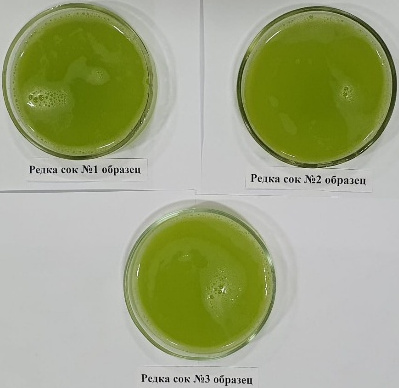
\includegraphics[width=0.8\textwidth]{media/pish/image58}
	\caption*{}
\end{figure}


\begin{figure}[H]
	\centering
	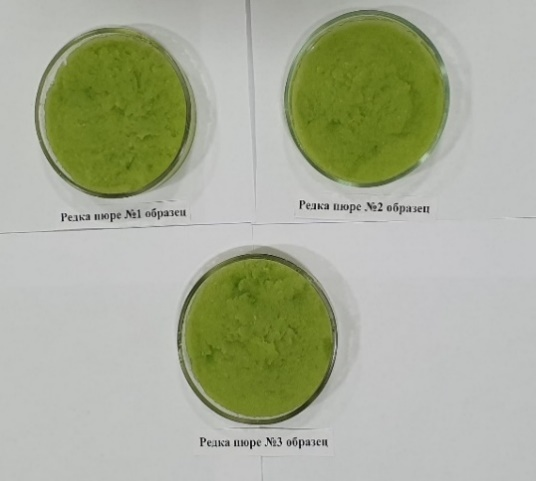
\includegraphics[width=0.8\textwidth]{media/pish/image59}
	\caption*{}
\end{figure}


\begin{figure}[H]
	\centering
	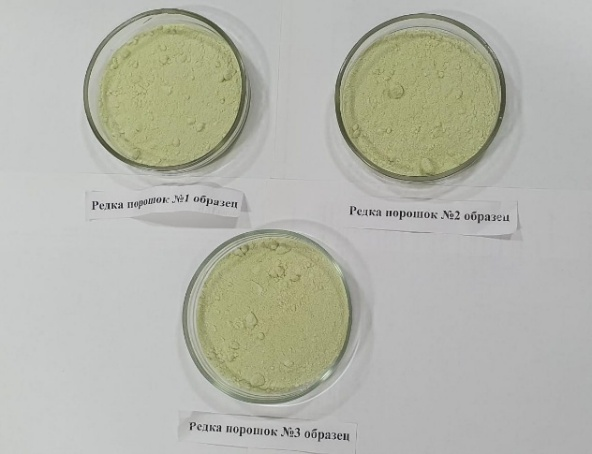
\includegraphics[width=0.8\textwidth]{media/pish/image60}
	\caption*{}
\end{figure}


а) б) в)

{\bfseries Рис.1 - Вид пюре, порошка и сока редьки:}

а) сок редьки; б) пюре редьки; в) порошок редьки

\begin{multicols}{2}
Второй этап -- явилось приготовление теста. За основу была выбрана
рецептура хлеба пшеничного высшего сорта (ГОСТ 27842-88). Опытные пробы
готовили: контроль без добавления редьки (контроль), с дозировкой сока
редьки 5 \% (образец № 1), 10 \% (образец № 2), 15 \% (образец № 3); с
дозировкой пюре редьки 1 \% (образец № 4), 3\% (образец № 5), 5\%
(образец № 6); с дозировкой порошка редьки 1\% (образец № 7), 5 \%
(образец № 8), 10 \% (образец № 9), от общего количества воды, начальная
температура теста 19-21°С.

Замешивание в аппарате сбивного теста длилось 4 минуты при 500 оборотах
в минуту, само сбивание теста проводили в течение 1 мин 50 сек при
давлении камеры 4 МПа и конечном сбивании в течении 30 сек. Для
приготовления пшеничного теста применяли безопарный способ тестоведения
{[}14-16{]}. Рецептурные компоненты и их соотношение показаны в таблице
1. Анализ готовых изделий проводили через 4 часа после выпечки.

Далее было выявлено влияние сока, пюре и порошка из редьки на
физико-химические показатели теста и хлеба (таблица 2).

Из таблицы 2 видно, что с увеличением дозировки сока, пюре и порошка из
редьки увеличивается кислотность, что оказывает влияние на с пористости
изделий на 15,3, 31,25 и 1,9\% для сока, на 25,8, 31,25, уменьшение на
11,76\% для пюре, увеличение на 23,0, 31,25 и уменьшение на 11,76\% для
порошка редьки сравнению с контролем, что ведет к увеличению усвояемости
хлебобулочных изделий (рисунок 3).
\end{multicols}

{\bfseries Таблица 1 - Рецептура хлеба с добавлением сока, пюре и порошка из редьки}

%% \begin{longtable}[]{@{}
%%   >{\raggedright\arraybackslash}p{(\linewidth - 20\tabcolsep) * \real{0.1853}}
%%   >{\centering\arraybackslash}p{(\linewidth - 20\tabcolsep) * \real{0.1085}}
%%   >{\centering\arraybackslash}p{(\linewidth - 20\tabcolsep) * \real{0.0774}}
%%   >{\centering\arraybackslash}p{(\linewidth - 20\tabcolsep) * \real{0.0775}}
%%   >{\centering\arraybackslash}p{(\linewidth - 20\tabcolsep) * \real{0.0775}}
%%   >{\centering\arraybackslash}p{(\linewidth - 20\tabcolsep) * \real{0.0721}}
%%   >{\centering\arraybackslash}p{(\linewidth - 20\tabcolsep) * \real{0.0802}}
%%   >{\centering\arraybackslash}p{(\linewidth - 20\tabcolsep) * \real{0.0802}}
%%   >{\centering\arraybackslash}p{(\linewidth - 20\tabcolsep) * \real{0.0802}}
%%   >{\centering\arraybackslash}p{(\linewidth - 20\tabcolsep) * \real{0.0802}}
%%   >{\centering\arraybackslash}p{(\linewidth - 20\tabcolsep) * \real{0.0802}}@{}}
%% \toprule\noalign{}
%% \begin{minipage}[b]{\linewidth}\centering
%% {\bfseries Компоненты}
%% \end{minipage} & \begin{minipage}[b]{\linewidth}\centering
%% {\bfseries Контроль}
%% \end{minipage} & \begin{minipage}[b]{\linewidth}\centering
%% {\bfseries №1}
%% \end{minipage} & \begin{minipage}[b]{\linewidth}\centering
%% {\bfseries №2}
%% \end{minipage} & \begin{minipage}[b]{\linewidth}\centering
%% {\bfseries №3}
%% \end{minipage} & \begin{minipage}[b]{\linewidth}\centering
%% {\bfseries №4}
%% \end{minipage} & \begin{minipage}[b]{\linewidth}\centering
%% {\bfseries №5}
%% \end{minipage} & \begin{minipage}[b]{\linewidth}\centering
%% {\bfseries №6}
%% \end{minipage} & \begin{minipage}[b]{\linewidth}\centering
%% {\bfseries №7}
%% \end{minipage} & \begin{minipage}[b]{\linewidth}\centering
%% {\bfseries №8}
%% \end{minipage} & \begin{minipage}[b]{\linewidth}\centering
%% {\bfseries №9}
%% \end{minipage} \\
%% \midrule\noalign{}
%% \endhead
%% \bottomrule\noalign{}
%% \endlastfoot
%% Мука пшеничная 1 сорта, г & 950 & 950 & 950 & 950 & 950 & 950 & 950 &
%% 950 & 950 & 950 \\
%% Сок редьки, мл & - & 50 & 100 & 150 & - & - & - & - & - & - \\
%% Пюре редьки, г & - & - & - & - & 10 & 30 & 50 & - & - & - \\
%% Порошок редьки, г & - & - & - & - & - & - & - & 10 & 50 & 100 \\
%% Лимонная кислота, г & 5 & 5 & 5 & 5 & 5 & 5 & 5 & 5 & 5 & 5 \\
%% Соль, г & 15 & 15 & 15 & 15 & 15 & 15 & 15 & 15 & 15 & 15 \\
%% Вода, мл &
%% \multicolumn{10}{>{\centering\arraybackslash}p{(\linewidth - 20\tabcolsep) * \real{0.8139} + 18\tabcolsep}@{}}{%
%% Согласно расчетам} \\
%% \end{longtable}

{\bfseries Таблица 2 - Влияние сока, пюре и порошка из редьки на качество
готовых полуфабрикатов и хлеба}

%% \begin{longtable}[]{@{}
%%   >{\raggedright\arraybackslash}p{(\linewidth - 20\tabcolsep) * \real{0.1726}}
%%   >{\raggedright\arraybackslash}p{(\linewidth - 20\tabcolsep) * \real{0.1255}}
%%   >{\raggedright\arraybackslash}p{(\linewidth - 20\tabcolsep) * \real{0.0844}}
%%   >{\raggedright\arraybackslash}p{(\linewidth - 20\tabcolsep) * \real{0.0893}}
%%   >{\raggedright\arraybackslash}p{(\linewidth - 20\tabcolsep) * \real{0.0865}}
%%   >{\raggedright\arraybackslash}p{(\linewidth - 20\tabcolsep) * \real{0.0735}}
%%   >{\raggedright\arraybackslash}p{(\linewidth - 20\tabcolsep) * \real{0.0736}}
%%   >{\raggedright\arraybackslash}p{(\linewidth - 20\tabcolsep) * \real{0.0736}}
%%   >{\raggedright\arraybackslash}p{(\linewidth - 20\tabcolsep) * \real{0.0736}}
%%   >{\raggedright\arraybackslash}p{(\linewidth - 20\tabcolsep) * \real{0.0736}}
%%   >{\raggedright\arraybackslash}p{(\linewidth - 20\tabcolsep) * \real{0.0736}}@{}}
%% \toprule\noalign{}
%% \begin{minipage}[b]{\linewidth}\centering
%% {\bfseries Показатели}
%% \end{minipage} & \begin{minipage}[b]{\linewidth}\centering
%% {\bfseries Контроль}
%% \end{minipage} & \begin{minipage}[b]{\linewidth}\centering
%% {\bfseries №1}
%% \end{minipage} & \begin{minipage}[b]{\linewidth}\centering
%% {\bfseries №2}
%% \end{minipage} & \begin{minipage}[b]{\linewidth}\centering
%% {\bfseries №3}
%% \end{minipage} & \begin{minipage}[b]{\linewidth}\centering
%% {\bfseries №4}
%% \end{minipage} & \begin{minipage}[b]{\linewidth}\centering
%% {\bfseries №5}
%% \end{minipage} & \begin{minipage}[b]{\linewidth}\centering
%% {\bfseries №6}
%% \end{minipage} & \begin{minipage}[b]{\linewidth}\centering
%% {\bfseries №7}
%% \end{minipage} & \begin{minipage}[b]{\linewidth}\centering
%% {\bfseries №8}
%% \end{minipage} & \begin{minipage}[b]{\linewidth}\centering
%% {\bfseries №9}
%% \end{minipage} \\
%% \midrule\noalign{}
%% \endhead
%% \bottomrule\noalign{}
%% \endlastfoot
%% Выход теста, г & 324 & 342 & 354 & 360 & 388 & 392 & 371 & 334 & 371 &
%% 424 \\
%% Температура теста, °С & 23 & 23,1 & 25 & 23,1 & 22,4 & 24,7 & 24,7 &
%% 24,8 & 23,1 & 23,1 \\
%% Влажность теста, \% & 55 & 54,5 & 54,6 & 54,5 & 54,0 & 55,0 & 55,0 &
%% 52,6 & 52,8 & 52,8 \\
%% Кислотность теста, град & 4,8 & 4,8 & 5,0 & 5,0 & 5,8 & 6,0 & 6,0 & 6,0
%% & 5,6 & 5,6 \\
%% Выход хлеба, г & 264,0 & 284 & 274,18 & 299 & 313 & 321 & 295 & 266 &
%% 296 & 342 \\
%% Влажность хлеба, \% & 52,8 & 53,3 & 52,4 & 53,3 & 54,4 & 53,2 & 53,2 &
%% 52 & 51,6 & 51,6 \\
%% Кислотность хлеба, град & 3,8 & 3,4 & 4,2 & 4,2 & 3,6 & 3,8 & 3,8 & 3,8
%% & 3,8 & 3,8 \\
%% Удельный объем, см\textsuperscript{3} & 280 & 283 & 290 & 290 & 271 &
%% 280 & 280 & 373 & 380 & 379 \\
%% Пористость хлеба, \% & 54,3 & 63,1 & 74,5 & 53,2 & 70,4 & 74,1 & 48,9 &
%% 68,4 & 74,5 & 48,3 \\
%% \end{longtable}

Анализируя данные таблицы 3 можно заметить что образцы номер 2, 5, 8
являются оптимальными по причине увеличения пористости, удельного объема
и выхода готовой продукции. С внесением дозировки сока, пюре и порошка
из редьки изменялись органолептические показатели готовых изделий.
Выявляли зависимость изменения выпеченного изделия от дозировки
компонентов редьки (рисунок 3).

%% \begin{longtable}[]{@{}
%%   >{\centering\arraybackslash}p{(\linewidth - 2\tabcolsep) * \real{0.4239}}
%%   >{\centering\arraybackslash}p{(\linewidth - 2\tabcolsep) * \real{0.5761}}@{}}
%% \toprule\noalign{}
%% \begin{minipage}[b]{\linewidth}\centering
%% 
%%\begin{figure}[H]
%%	\centering
%%	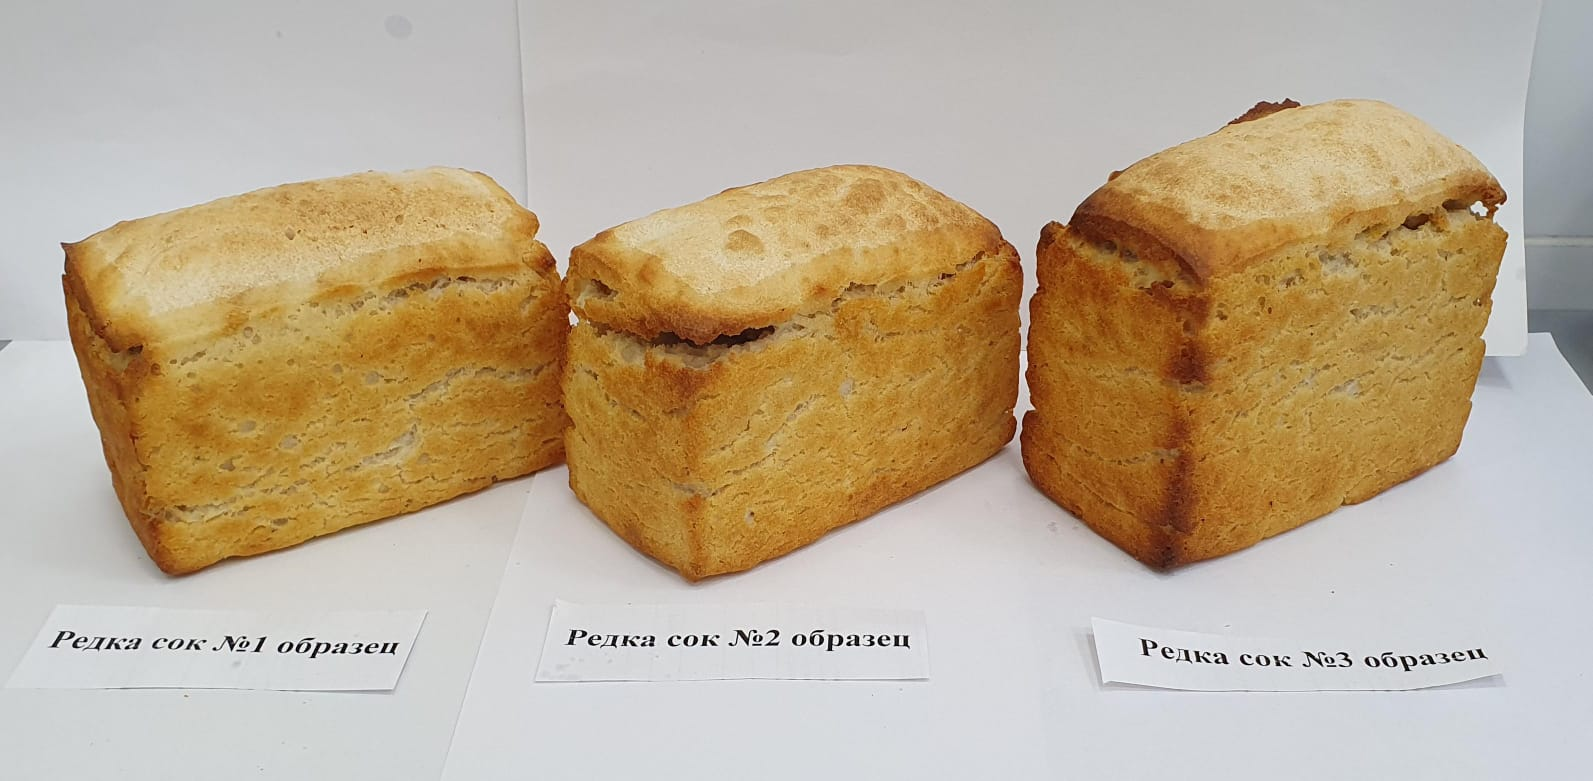
\includegraphics[width=0.8\textwidth]{media/pish/image61}
%%	\caption*{}
%%\end{figure}

%% \end{minipage} & \begin{minipage}[b]{\linewidth}\centering
%% 
%%\begin{figure}[H]
%%	\centering
%%	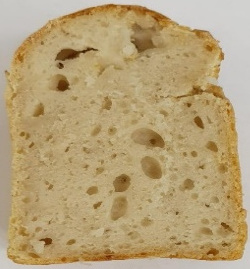
\includegraphics[width=0.8\textwidth]{media/pish/image62}
%%	\caption*{}
%%\end{figure}

%% а)
%% \end{minipage} \\
%% \midrule\noalign{}
%% \endhead
%% \bottomrule\noalign{}
%% \endlastfoot
%% 
%%\begin{figure}[H]
%%	\centering
%%	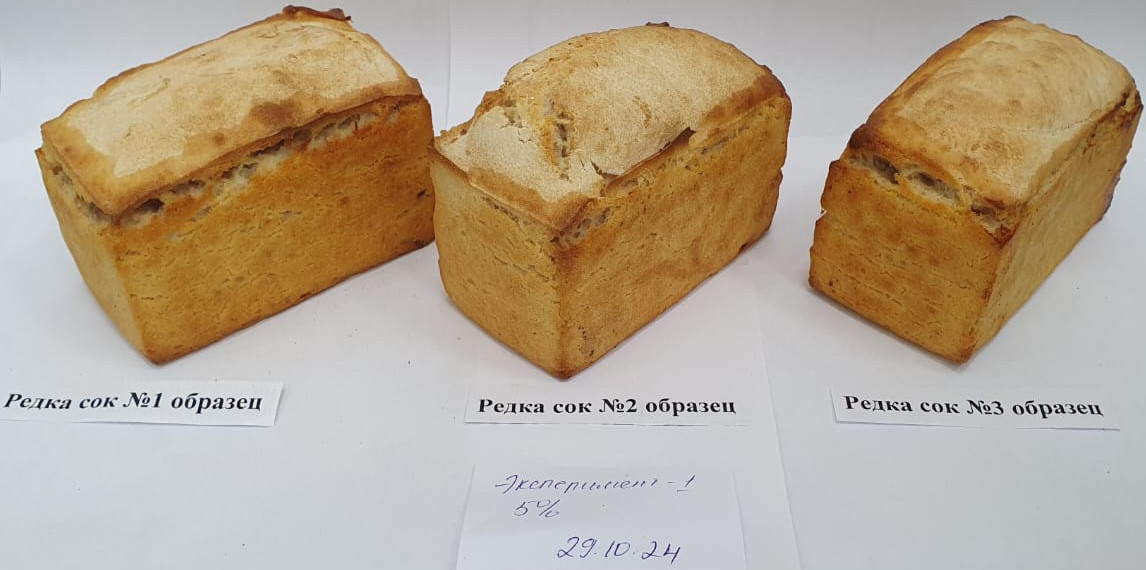
\includegraphics[width=0.8\textwidth]{media/pish/image63}
%%	\caption*{}
%%\end{figure}
%% &
%% 
%%\begin{figure}[H]
%%	\centering
%%	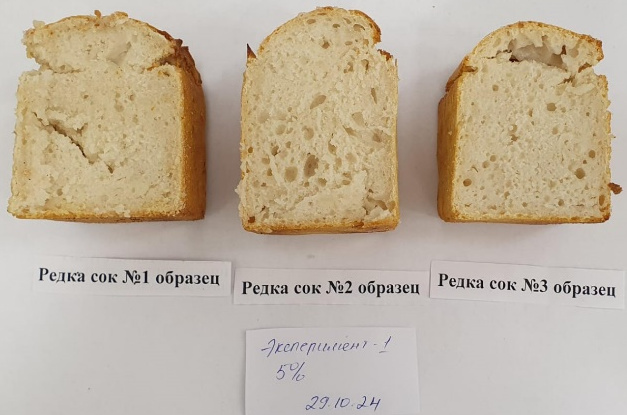
\includegraphics[width=0.8\textwidth]{media/pish/image64}
%%	\caption*{}
%%\end{figure}

%% б) \\
%% 
%%\begin{figure}[H]
%%	\centering
%%	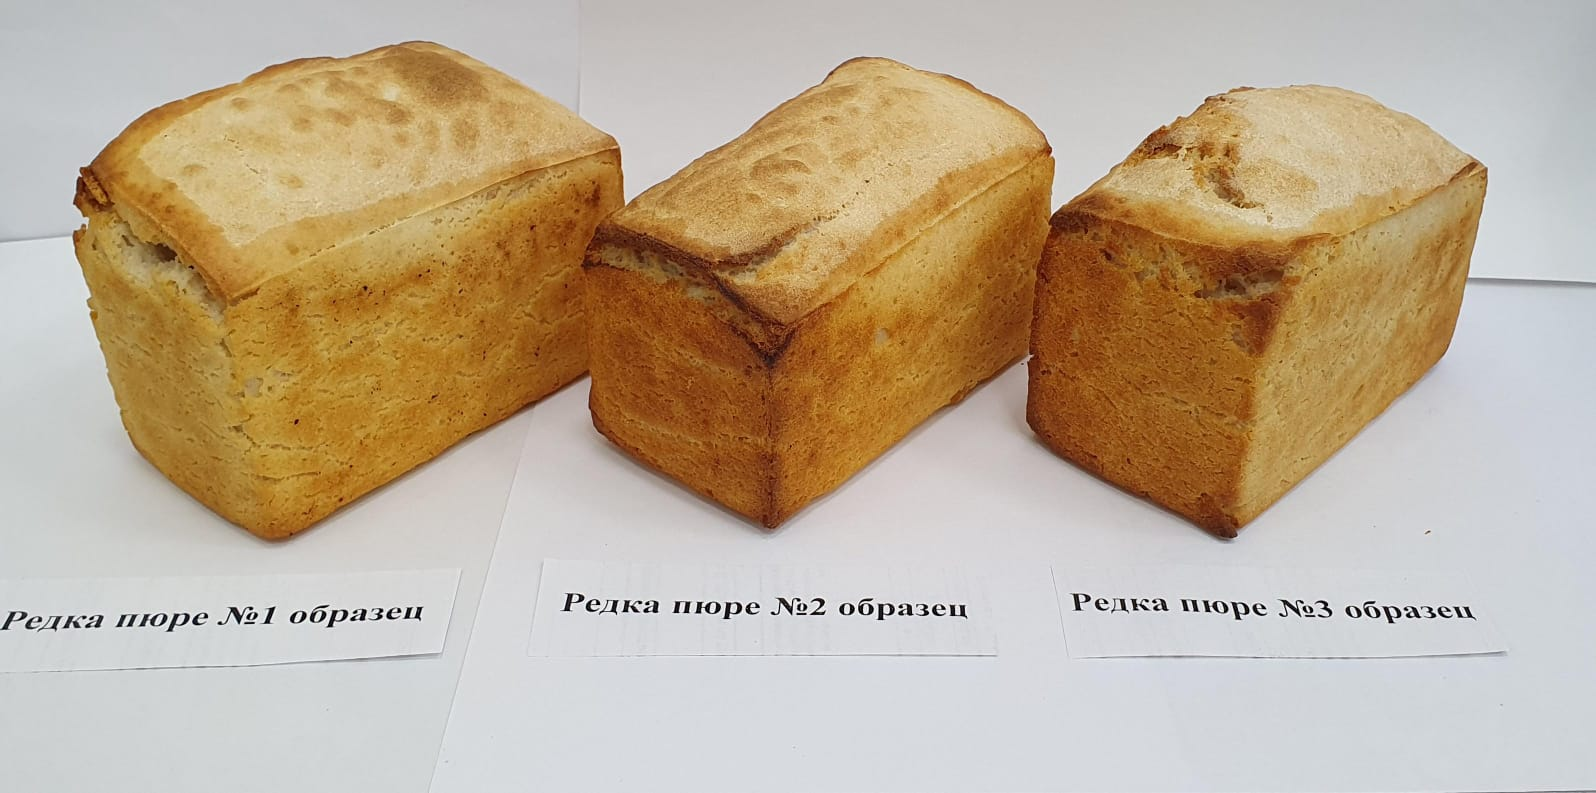
\includegraphics[width=0.8\textwidth]{media/pish/image65}
%%	\caption*{}
%%\end{figure}
 %%&
%% 
%%\begin{figure}[H]
%%	\centering
%%	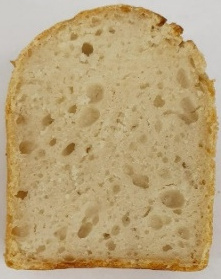
\includegraphics[width=0.8\textwidth]{media/pish/image66}
%%	\caption*{}
%%\end{figure}

%% в) \\
%% 
%%\begin{figure}[H]
%%	\centering
%%	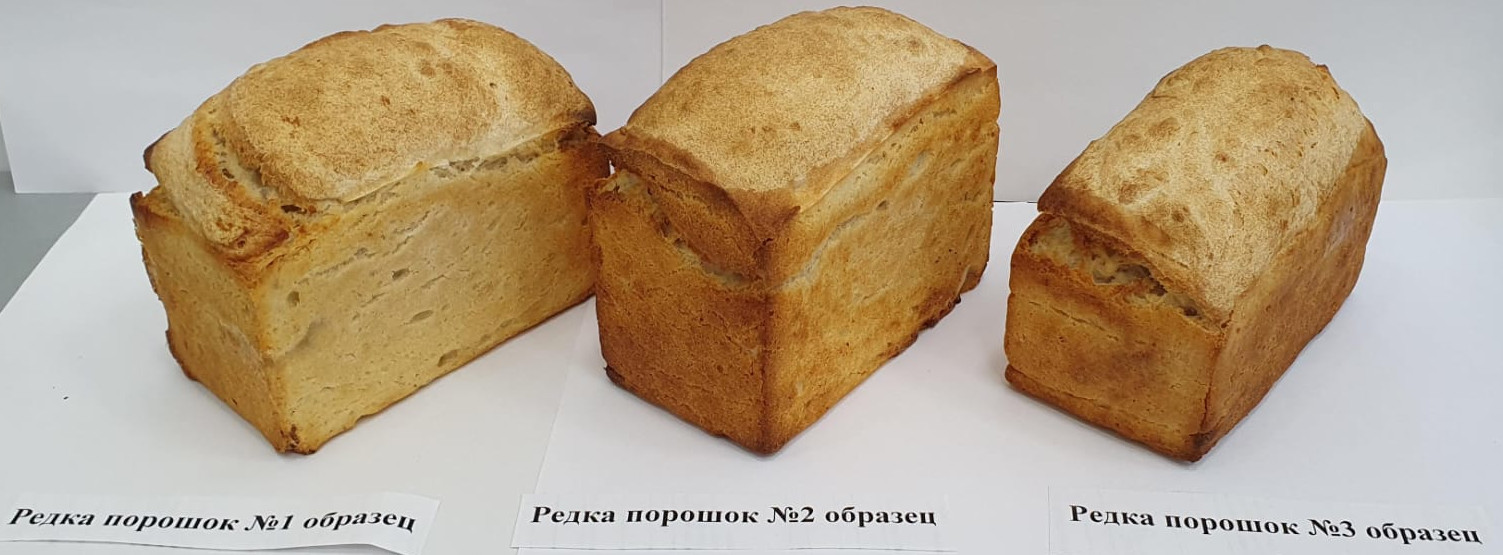
\includegraphics[width=0.8\textwidth]{media/pish/image67}
%%	\caption*{}
%%\end{figure}
 %%&
%% 
%% \begin{figure}[H]
%% 	\centering
%% 	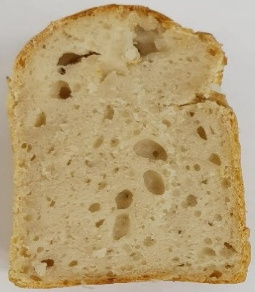
\includegraphics[width=0.8\textwidth]{media/pish/image68}
%%	\caption*{}
%%\end{figure}

%% г) \\
%% \end{longtable}

{\bfseries Рис.2 - Вид образцов хлеба с добавлением сока, пюре и порошка редьки:}

а) контроль, б) с дозировкой сока редьки; в) с дозировкой пюре редьки;

г) с дозировкой порошка редьки

\begin{multicols}{2}
Полученные результаты органолептической оценки позволяют сказать, что
контрольные и опытные образцы хлебобулочных изделий имели правильную
форму, гладкую поверхность, равномерную пористость, достаточную
эластичность мякиша. Образцами с лучшими показателями оказались образцы
с добавлением порошка редьки, худшими -- с добавлением пюре редьки.
Добавление порошка редьки значительно улучшило пористость, объем хлеба и
структуру мякиша по сравнению не только с контрольным, но и с другими
образцами хлеба с добавлением компонентов редьки.
\end{multicols}

{\bfseries Рис.3 - Органолептические показатели хлеба с добавлением сока,
пюре и порошка редьки}

\begin{multicols}{2}
Эластичность мякиша контрольных образцов имела наименьшие значения,
дегустаторы отмечали повышенную плотность и комкающийся мякиш, что
наиболее ощущалось на конец хранения. При этом опытные образцы,
полученные с внесением порошка редьки, характеризовались более
равномерной тонкостенной развитой пористостью, мягким, достаточно
эластичным мякишем с хорошей разжевываемостью.

Опытные образцы, полученные с внесением редьки, имели наилучшие свойства
мякиша: мягкий, эластичный, хорошо разжевываемый, создающий приятное
ощущение (вкус и аромат) во рту по сравнению с контрольным образцом.
Основываясь на предыдущих результатах экспериментов, для дальнейших
исследований были отобраны следующие образцы: 2, 5 и 8, как образцы,
имеющие лучшие показатели по сравнению с контрольным образцом. Далее
были проведены некоторые физико-химические, биохимические,
микробиологические показатели хлеба с добавлением сока, пюре и порошка
редьки (таблица 3 и 4).
\end{multicols}

{\bfseries Таблица 3 - Влияние сока, пюре и порошка редьки на физико-химические показатели хлеба}

%% \begin{longtable}[]{@{}
%%   >{\centering\arraybackslash}p{(\linewidth - 8\tabcolsep) * \real{0.3332}}
%%   >{\centering\arraybackslash}p{(\linewidth - 8\tabcolsep) * \real{0.1668}}
%%   >{\centering\arraybackslash}p{(\linewidth - 8\tabcolsep) * \real{0.1517}}
%%   >{\centering\arraybackslash}p{(\linewidth - 8\tabcolsep) * \real{0.1820}}
%%   >{\centering\arraybackslash}p{(\linewidth - 8\tabcolsep) * \real{0.1662}}@{}}
%% \toprule\noalign{}
%% \begin{minipage}[b]{\linewidth}\centering
%% {\bfseries Показатели}
%% \end{minipage} & \begin{minipage}[b]{\linewidth}\centering
%% {\bfseries Контроль}
%% \end{minipage} & \begin{minipage}[b]{\linewidth}\centering
%% {\bfseries №2}
%% \end{minipage} & \begin{minipage}[b]{\linewidth}\centering
%% {\bfseries №5}
%% \end{minipage} & \begin{minipage}[b]{\linewidth}\centering
%% {\bfseries №8}
%% \end{minipage} \\
%% \midrule\noalign{}
%% \endhead
%% \bottomrule\noalign{}
%% \endlastfoot
%% Мас.доля белка, \% & 6,92 & 7,87 & 6,94 & 7,50 \\
%% Мас.доля жира, \% & 0,52 & 0,77 & 0,64 & 0,82 \\
%% Мас.доля углеводов, \% & 23,30 & 27,70 & 25,65 & 26,04 \\
%% Мас.доля пищевых волокон (клетчатка), \% & 4,71 & 4,95 & 5,56 & 6,04 \\
%% \end{longtable}

Судя по полученным данным, по сравнению с контрольным образцом в соке
редьки на 13,72\% больше белка, в порошке редьки данный показатель
увеличивается на 8,38\%. Содержание пищевых волокон также значительно
увеличивается в образцах с добавлением сока, пюре и порошка из редьки.
Так, добавление порошка редьки увеличивает на 28,23\%, пюре на 18,04\%,
а сока на 5,09\% содержание пищевых волокон в хлебе. Во всех образцах с
редькой есть не большое увеличение содержания жира и углеводов.

{\bfseries Таблица 3 - Влияние сока, пюре и порошка редьки на
биохимические показатели хлеба и содержание тяжелых элементов в хлебе}

%% \begin{longtable}[]{@{}
%%   >{\raggedright\arraybackslash}p{(\linewidth - 8\tabcolsep) * \real{0.2421}}
%%   >{\centering\arraybackslash}p{(\linewidth - 8\tabcolsep) * \real{0.1972}}
%%   >{\centering\arraybackslash}p{(\linewidth - 8\tabcolsep) * \real{0.1972}}
%%   >{\centering\arraybackslash}p{(\linewidth - 8\tabcolsep) * \real{0.1634}}
%%   >{\centering\arraybackslash}p{(\linewidth - 8\tabcolsep) * \real{0.2000}}@{}}
%% \toprule\noalign{}
%% \begin{minipage}[b]{\linewidth}\centering
%% {\bfseries Показатели}
%% \end{minipage} & \begin{minipage}[b]{\linewidth}\centering
%% {\bfseries Контроль}
%% \end{minipage} & \begin{minipage}[b]{\linewidth}\centering
%% {\bfseries №2}
%% \end{minipage} & \begin{minipage}[b]{\linewidth}\centering
%% {\bfseries №5}
%% \end{minipage} & \begin{minipage}[b]{\linewidth}\centering
%% {\bfseries №8}
%% \end{minipage} \\
%% \midrule\noalign{}
%% \endhead
%% \bottomrule\noalign{}
%% \endlastfoot
%% {\bfseries Витамины:}
%% 
%% А, мг/кг &
%% \multicolumn{4}{>{\centering\arraybackslash}p{(\linewidth - 8\tabcolsep) * \real{0.7579} + 6\tabcolsep}@{}}{%
%% нe oбнаружено} \\
%% Е, мг/кг &
%% \multicolumn{4}{>{\centering\arraybackslash}p{(\linewidth - 8\tabcolsep) * \real{0.7579} + 6\tabcolsep}@{}}{%
%% нe oбнаружено} \\
%% В\textsubscript{1}, мг / 100 г & 0,04 & 0,05 & 0,06 & 0,03 \\
%% В\textsubscript{2}, мг / 100 г & 0,01 & 0,01 & 0,02 & 0,01 \\
%% В\textsubscript{3}, мг / 100 г & 1,53 & 1,65 & 1,60 & 1,50 \\
%% В\textsubscript{5}, мг / 100 г & 0,50 & 0,68 & 0,54 & 0,41 \\
%% В\textsubscript{6}, мг / 100 г & 0,10 & 0,13 & 0,12 & 0,09 \\
%% Вс, мг / 100 г &
%% \multicolumn{4}{>{\centering\arraybackslash}p{(\linewidth - 8\tabcolsep) * \real{0.7579} + 6\tabcolsep}@{}}{%
%% нe oбнаружено} \\
%% С, мг / 100 г & нe oбнаружено & l,90 & 1,64 & 1,08 \\
%% {\bfseries Минеральные элементы:}
%% 
%% железо, мг / 100 г & 2,70 & 2,85 & 2,80 & 3,05 \\
%% калий, мг / 100 г & 156,98 & 173,2 & 170,7 & 124,6 \\
%% кальций, мг / 100 г & 24,63 & {\bfseries 30,29} & 25,18 & 23,01 \\
%% магний, мг / 100 г & 18,17 & 19,94 & 21,85 & 18,25 \\
%% фосфор, мг / 100 г & 90,19 & {\bfseries 100,13} & 95,84 & 80,38 \\
%% натрий, мг / 100 г & 348,94 & 371,85 & 385,13 & 381,46 \\
%% {\bfseries Токсичные элементы:}
%% 
%% свинец, мг/кг &
%% \multicolumn{4}{>{\centering\arraybackslash}p{(\linewidth - 8\tabcolsep) * \real{0.7579} + 6\tabcolsep}@{}}{%
%% нe oбнаружено} \\
%% кадмий, мг/кг &
%% \multicolumn{4}{>{\centering\arraybackslash}p{(\linewidth - 8\tabcolsep) * \real{0.7579} + 6\tabcolsep}@{}}{%
%% нe oбнаружено} \\
%% мышьяк, мг/кг &
%% \multicolumn{4}{>{\centering\arraybackslash}p{(\linewidth - 8\tabcolsep) * \real{0.7579} + 6\tabcolsep}@{}}{%
%% нe oбнаружено} \\
%% \end{longtable}

Анализируя полученные данные, можно отметить повышение по ряду
показателей. Так, если в контрольном образце не был обнаружен витамин С,
то в образцах с добавлением редьки, он присутствует в значительном
объеме, а витамины группы В в хлебе с соком и пюре редьки по сравнению с
контрольным образцом содержаться на 50-100\% больше. Но в хлебе с
содержанием порошка редьки замечено, что содержание витаминов группы В
уменьшается благодаря высушиванию, т.е. обработке небольшим термическим
воздействием.

Были замечены значительные изменения по содержанию микро-
макроэлементов, в особенности натрий в пюре увеличилось на 10,37\%,
калия в хлебе с соком редьки увеличилось на 10,33\%, фосфора в хлебе с
соком редьки 11,02\%, кальция в хлебе с соком редьки на 31,63\%, железо
в хлебе с пюре редьки на 7,01\% по сравнению с контрольным образцом.
Токсичным элементов, таких как свинец, кадмий и мышьяк во всех образцах
не было обнаружено.

{\bfseries Таблица 4 -- Влияние сока, пюре и порошка редьки на
микробиологические показатели хлеба}

%% \begin{longtable}[]{@{}
%%   >{\centering\arraybackslash}p{(\linewidth - 8\tabcolsep) * \real{0.3484}}
%%   >{\centering\arraybackslash}p{(\linewidth - 8\tabcolsep) * \real{0.1820}}
%%   >{\centering\arraybackslash}p{(\linewidth - 8\tabcolsep) * \real{0.1668}}
%%   >{\centering\arraybackslash}p{(\linewidth - 8\tabcolsep) * \real{0.1516}}
%%   >{\centering\arraybackslash}p{(\linewidth - 8\tabcolsep) * \real{0.1511}}@{}}
%% \toprule\noalign{}
%% \begin{minipage}[b]{\linewidth}\centering
%% {\bfseries Показатели}
%% \end{minipage} & \begin{minipage}[b]{\linewidth}\centering
%% {\bfseries Контроль}
%% \end{minipage} & \begin{minipage}[b]{\linewidth}\centering
%% {\bfseries №2}
%% \end{minipage} & \begin{minipage}[b]{\linewidth}\centering
%% {\bfseries №5}
%% \end{minipage} & \begin{minipage}[b]{\linewidth}\centering
%% {\bfseries №8}
%% \end{minipage} \\
%% \midrule\noalign{}
%% \endhead
%% \bottomrule\noalign{}
%% \endlastfoot
%% КМАФАнМ, КОЕ/г & 3x10\textsuperscript{2} & 3x10\textsuperscript{2} &
%% 7x10\textsuperscript{2} & 4x10\textsuperscript{2} \\
%% БГКП (колиформы) в 1,0 см\textsuperscript{3} продукта &
%% \multicolumn{4}{>{\centering\arraybackslash}p{(\linewidth - 8\tabcolsep) * \real{0.6516} + 6\tabcolsep}@{}}{%
%% нe oбнаружено} \\
%% \end{longtable}

\begin{multicols}{2}
Микробиологические показатели, показанные в таблице 4 во всех образцах
хлеба были в норме. БГКП во всех образцах не были обнаружены. Таким
образом, все образцы хлеба безопасны для употребления человеком по
микробиологическим показателям и содержанию токсичных элементов.

{\bfseries Выводы}. Таким образом, применение сбивной технологии уменьшило
время, традиционно затрачиваемое на приготовление теста, а образом,
примнение сбивной технологии уменьшило время, традиционно затрачиваемое
на приготовление теста, а анализируя все полученные экспериментальные
данные, можно сделать вывод о том, что добавление сока, пюре и порошка
редьки значительно повышают пищевую и биологическую ценность как
полуфабрикатов, так и готового хлеба. Значительно повышается содержание
пищевой клетчатки, белка, микро- макроэлементов и витаминов, при том,
что сохраняется микробиологическая и токсикологическая ценность готовых
образцов хлеба. Также замечено значительное улучшение реологических и
потребительских свойств хлеба. В особенности в хлебе с добавлением
порошка редьки (увеличение пор мякиша, объема хлеба, структуры мякиша,
эластичности и т.д.). Если рассматривать различия и эффективность
применения сока, пюре и порошка редьки по содержанию нутриентов, то
можно сделать вывод о том, что добавление порошка и сока редьки
значительно более привлекательны по реологическим свойствам, по
содержанию витаминов, микро- макроэлементов по сравнению с хлебом с
добавлением пюре редьки.

Полученные данные показывают эффективность применения сока, пюре и
порошки редьки в хлебопечении: увеличилось содержание натрия в хлебе с
пюре редьки увеличилось на 10,37\%, калия в хлебе с соком редьки
увеличилось на 10,33\%, фосфора в хлебе с соком редьки 11,02\%, кальция
в хлебе с соком редьки на 31,63\%, железо в хлебе с пюре редьки на
7,01\% по сравнению с контрольным образцом. Содержание пищевых волокон в
хлебе с порошком редьки увеличивается на 28,23\%, пюре на 18,04\%, а
сока на 5,09\% содержание пищевых волокон в хлебе. Таким образом,
разработанная инновационная технология бездрожжевого хлеба из сбивного
теста с добавлением сока, пюре и порошка редьки является
высокоперспективной и рекомендуется для внедрения в хлебопечение, в том
числе как профилактическое и диетическое средство.

\emph{{\bfseries Финансирование}. Данная статья была подготовлена в рамках
проекта №AP23490384 "Разработка инновационной технологии ускоренного
приготовления замороженного теста, обогащенного растительными
культурами".}
\end{multicols}

\begin{center}
{\bfseries Литература}
\end{center}

\begin{references}
1. Thuengtung S., Ogawa Y. Comparative study of conventional steam
cooking and microwave cooking on cooked pigmented rice texture and their
phenolic antioxidant // Food Science and Nutrition. -2020.- Vol.8(20.-
P.965--972. DOI 10.1002/fsn3.1377.

2. О мерах по обеспечению рационального использования продовольственных
ресурсов в Республике Казахстан {[}Электронный ресурс{]}. -- URL:
\url{https://adilet.zan.kz/rus/docs/V1600014674} .-Lата обращения:
05.03.2015.3.Тутельян В.А. Химический состав и калорийность российских продуктов
питания: {[}Справочник{]}. -- М.: ДеЛи плюс, 2012. - 284 с.ISBN
978-5-905170-20-1

4. Сафарова Г.А., Кароматов И.Д. Лечебные свойства растения редька //
Биология и интегративная медицина. -- 2018. -- № 6. -- С.174--187.

5. Донченко Л.В., Сокол Н.В., Влащик Л.Г. Обогащение хлеба биологически
активными веществами профилактического назначения // Научный журнал
КубГАУ. -- 2017. -- № 125. -- С.597--610.

6. Пат.2370959 РФ, C1. Способ производства сбивного бездрожжевого хлеба
/ Магомедов Г.О., Пономарева Е.И., Алейник И.А., Лобосов В.Г., Сарыева
А.Г.; заявитель и патентообладатель ФГБОУ ВО «Кубанский государственный
аграрный университет». -- № 2008108527/13; заявл.03.03.2008; опубл.
27.10.2009, Бюл. № 30.

7. Пат.2380907 РФ, C1. Способ производства сбивного бездрожжевого хлеба
повышенной пищевой ценности / Магомедов Г.О., Пономарева Е.И., Алейник
И.А., Воропаева О.Н.; заявитель и патентообладатель ФГБОУ ВО «Кубанский
государственный аграрный университет». -- № 2009138031/13; заявл.
13.10.2009; опубл.10.02.2010, Бюл. № 4.

8. Печерских Р.Т., Фролов Д.В., Шахов С.В., Рыженин П.Ю., Таратухин А.С.
Способ производства сбивного бездрожжевого хлеба из муки цельносмолотого
зерна пшеницы // Современные наукоемкие технологии. -- 2014. -- № 5-1.
-- С.165.

9. Магомедов Г.О., Лукина С.И., Садыгова М.К., Вавилова А.А. Разработка
технологии сбивного хлеба из нутовой муки // Современные наукоемкие
технологии. -- 2014. -- № 12-1. -- С.113.

10. Магомедов Г.О., Пономарева Е.И., Алейник И.А. Инновационные
технологии сбивных бездрожжевых хлебобулочных изделий функционального
назначения // Фундаментальные исследования. -- 2008. -- № 1. -- С.
71--72.

11. Kumar С., Karim M.A. Microwave-convective drying of food materials: A
critical review // Critical Reviews in Food Science and Nutrition. --
2019. - Vol.59(3).- P.379--394.
\href{https://doi.org/10.1080/10408398.2017.1373269}{DOI\\
10.1080/10408398.2017.1373269}.

12. Кулишов Б.А., Новоселов А.Г., Иващенко С.Ю., Гусаров Н.Е. Применение
электроконтактного нагрева в хлебопечении: обзор // Ползуновский
вестник. -- 2019. -- № 1. -- С.106--113.DOI\\
10.25712/ASTU.2072-8921.2019.01.020

13. Дзантиева Е.Э., Лыгин В.В., Миронова Е.О. и др. Микробиологические
показатели сбивного хлеба «крестьянский» из тритикалевой муки //
Молодежный инновационный вестник. - 2016. -Т.5(1). - С.427-428.

14. Садыгова М.К., Буховец В.А., Бороздина А.В. и др. Разработка
технологических решений использования продуктов переработки из
корнеплодов в производстве бисквита // Естественные и технические науки.
- 2018.- № 3(117). -- С.109--113.

15. Малышев В.К., Демидова Т.И., Нечаев А.П. и др. Функциональные
продукты питания: особенности современного развития пищевых технологи//
Хранение и переработка сельхозсырья. - 2012.-№ 6. - С.51--52.

16. Kalla A.M., Devaraju R. Microwave energy and its application in food
industry: A review // Asian Journal of Dairy and Food Research.- 2017.-
Vol.36(1).- P.37--44.
\href{https://doi.org/10.18805/ajdfr.v0iOF.7303}{DOI
10.18805/ajdfr.v0iOF.7303}.
\end{references}

\begin{center}
{\bfseries References}
\end{center}

\begin{references}
1. Thuengtung S., Ogawa Y. Comparative study of conventional steam
cooking and microwave cooking on cooked pigmented rice texture and their
phenolic antioxidant // Food Science and Nutrition. -2020.- Vol.8(20.-
P.965--972. DOI 10.1002/fsn3.1377.

2. O merah po obespecheniju racional' nogo
ispol' zovanija prodovol' stvennyh
resursov v Respublike Kazahstan {[}Jelektronnyj resurs{]}. -- URL:
https://adilet.zan.kz/rus/docs/V1600014674 .-Lata obrashhenija:
05.03.2015. {[}in Russian{]}

3. Tutel' jan V.A. Himicheskij sostav i
kalorijnost'{} rossijskih produktov pitanija:
{[}Spravochnik{]}. -- M.: DeLi pljus, 2012. - 284 s.ISBN
978-5-905170-20-1.{[}in Russian{]}

4. Safarova G.A., Karomatov I.D. Lechebnye svojstva rastenija
red' ka // Biologija i integrativnaja medicina. -- 2018.
-- № 6. -- S.174--187.{[}in Russian{]}

5. Donchenko L.V., Sokol N.V., Vlashhik L.G. Obogashhenie hleba
biologicheski aktivnymi veshhestvami profilakticheskogo naznachenija //
Nauchnyj zhurnal KubGAU. -- 2017. -- № 125. -- S.597--610. {[}in
Russian{]}

6. Pat.2370959 RF, C1. Sposob proizvodstva sbivnogo bezdrozhzhevogo
hleba / Magomedov G.O., \\Ponomareva E.I., Alejnik I.A., Lobosov V.G.,
Saryeva A.G.; zajavitel'{} i
patentoobladatel'{} FGBOU VO «Kubanskij gosudarstvennyj
agrarnyj universitet». -- № 2008108527/13; zajavl.03.03.2008; opubl.\\
27.10.2009, Bjul. № 30. {[}in Russian{]}

7. Pat.2380907 RF, C1. Sposob proizvodstva sbivnogo bezdrozhzhevogo
hleba povyshennoj pishhevoj cennosti / Magomedov G.O., Ponomareva E.I.,
Alejnik I.A., Voropaeva O.N.; zajavitel'{} i
patentoobladatel'{} FGBOU VO «Kubanskij gosudarstvennyj
agrarnyj universitet». -- № 2009138031/13; zajavl.13.10.2009; opubl.
10.02.2010, Bjul. № 4. {[}in Russian{]}

8. Pecherskih R.T., Frolov D.V., Shahov S.V., Ryzhenin P.Ju., Taratuhin
A.S. Sposob proizvodstva sbivnogo bezdrozhzhevogo hleba iz muki
cel' nosmolotogo zerna pshenicy // Sovremennye naukoemkie
tehnologii. -- 2014. -- № 5-1. -- S.165. {[}in Russian{]}

9. Magomedov G.O., Lukina S.I., Sadygova M.K., Vavilova A.A. Razrabotka
tehnologii sbivnogo hleba iz nutovoj muki // Sovremennye naukoemkie
tehnologii. -- 2014. -- № 12-1. -- S.113. {[}in Russian{]}

10. Magomedov G.O., Ponomareva E.I., Alejnik I.A. Innovacionnye
tehnologii sbivnyh bezdrozhzhevyh hlebobulochnyh izdelij
funkcional' nogo naznachenija //
Fundamental' nye issledovanija. -- 2008. -- № 1. -- S.
71--72. {[}in Russian{]}

11. Kumar С., Karim M.A. Microwave-convective drying of food materials: A
critical review // Critical Reviews in Food Science and Nutrition. --
2019. - Vol.59(3).- P.379--394.
\href{https://doi.org/10.1080/10408398.2017.1373269}{DOI\\
10.1080/10408398.2017.1373269}.

12. Kulishov B.A., Novoselov A.G., Ivashhenko S.Ju., Gusarov N.E.
Primenenie jelektrokontaktnogo nagreva v hlebopechenii: obzor //
Polzunovskij vestnik. -- 2019. -- № 1. -- S.106--113.DOI\\
10.25712/ASTU.2072-8921.2019.01.020. {[}in Russian{]}

13. Dzantieva E.Je., Lygin V.V., Mironova E.O. i dr. Mikrobiologicheskie
pokazateli sbivnogo hleba «krest' janskij» iz
tritikalevoj muki // Molodezhnyj innovacionnyj vestnik. - 2016. -T.
5(1). - S.427-428. {[}in Russian{]}

14. Sadygova M.K., Buhovec V.A., Borozdina A.V. i dr. Razrabotka
tehnologicheskih reshenij ispol' zovanija produktov
pererabotki iz korneplodov v proizvodstve biskvita // Estestvennye i
tehnicheskie nauki. - 2018.- № 3(117). -- S.109--113. {[}in Russian{]}

15. Malyshev V.K., Demidova T.I., Nechaev A.P. i dr.
Funkcional' nye produkty pitanija: osobennosti
sovremennogo razvitija pishhevyh tehnologi// Hranenie i pererabotka
sel' hozsyr' ja. - 2012.-№ 6. - S.51--52.
{[}in Russian{]}

16. Kalla A.M., Devaraju R. Microwave energy and its application in food
industry: A review // Asian Journal of Dairy and Food Research.- 2017.-
Vol.36(1).- P.37--44.
\href{https://doi.org/10.18805/ajdfr.v0iOF.7303}{DOI
10.18805/ajdfr.v0iOF.7303}.
\end{references}

\begin{authorinfo}
\emph{{\bfseries Сведения об авторах}}

Турсунбаева Ш.А.- доктор философских наук (Ph.D), и. о. ассоциированного
профессора, АО "Алматинский технологический университет", Алматы,
Казахстан, e-mail:
\href{mailto:sh.tursunbaeva@bk.ru}{\nolinkurl{sh.tursunbaeva@bk.ru}};
\url{https://orcid.org/0000-0001-9645-3634}

Изтаев А.И.- доктор технических наук, профессор, академик НАН, АО
"Алматинский технологический университет", Алматы, Казахстан, e-mail:
\href{mailto:auelbekking@mail.ru}{\nolinkurl{auelbekking@mail.ru}};
\url{https://orcid.org/0000-0002-7385-482X}

Якияева М.А.- доктор философии (Ph.D), ассоциированный профессор, АО
«Алматинский технологический университет», Алматы, Казахстан, e-mail:
\href{mailto:yamadina88@mail.ru}{\nolinkurl{yamadina88@mail.ru}};
\url{https://orcid.org/0000-0002-8564-2912}

Мулдабекова Б.Ж.-доктор технических наук, профессор, АО "Алматинский
технологический университет", e-mail: Алматы, Казахстан,
\href{mailto:bayan\_1004@mail.ru}{\nolinkurl{bayan\_1004@mail.ru}};
\url{https://orcid.org/0000-0003-1848-4288}

Нургожина Ж.К.- доктор философских наук (Ph.D), ассистент-профессор, АО
"Алматинский технологический университет", Алматы, Казахстан, e-mail:
\href{mailto:juldyz\_900@mail.ru}{\nolinkurl{juldyz\_900@mail.ru}}.
\url{https://orcid.org/0000-0002-6576-4445}

\emph{{\bfseries Information about authors}}

Tursunbayeva Sh. A. - Doctor of Philosophy (Ph.D), Acting. Associate
Professor, JSC "Almaty Technological University", Almaty, Kazakhstan,
e-mail:
\href{mailto:sh.tursunbaeva@bk.ru}{\nolinkurl{sh.tursunbaeva@bk.ru}};

Iztayev A.I. - Doctor of Technical Sciences, Professor, Academician of
the National Academy of Sciences, JSC "Almaty Technological University",
Almaty, Kazakhstan, e-mail:
\href{mailto:auelbekking@mail.ru}{\nolinkurl{auelbekking@mail.ru}};

Yakiyayeva M.A. - Doctor of Philosophy (Ph.D), Associate Professor, JSC
"Almaty Technological University", Almaty, \\Kazakhstan, e-mail:
\href{mailto:yamadina88@mail.ru}{\nolinkurl{yamadina88@mail.ru}};

Muldabekova Bayan Zhaksylykovna - Doctor of Technical Sciences,
Professor, JSC "Almaty Technological University", Almaty, Kazakhstan,
e-mail:
\href{mailto:bayan\_1004@mail.ru}{\nolinkurl{bayan\_1004@mail.ru}};

Nurgozina Zhuldyz Kanatovna - Doctor of Philosophy (Ph.D), Assistant
Professor, JSC "Almaty Technological University", Almaty, Kazakhstan,
e-mail:\href{mailto:juldyz\_900@mail.ru}{\nolinkurl{juldyz\_900@mail.ru}}
\end{authorinfo}
